\documentclass[aspectratio=169]{beamer}

% fix scr error
\usepackage{scrhack}
%%%%%%%%%%%%%%%%%%%%%%%%%%%%%%
% Kopf- und Fußzeilen definieren
%%%%%%%%%%%%%%%%%%%%%%%%%%%%%%
\usepackage[autooneside = false]{scrlayer-scrpage}
    \ohead{\headmark}
    \ofoot{\pagemark}
    \automark[section]{chapter}
    \renewcommand{\autodot}{}
    \addtokomafont{pagenumber}{\bfseries}
	\addtokomafont{disposition}{\rmfamily}

%%%%%%%%%%%%%%%%%%%%%%%%%%%%%%
% Um ToDos einfügen zu können
%%%%%%%%%%%%%%%%%%%%%%%%%%%%%%
\usepackage[linecolor=myyellow,backgroundcolor = myyellow]{todonotes}

%%%%%%%%%%%%%%%%%%%%%%%%%%%%%%
%Sprach-, Schrift- und Formatierungseinstellungen
%%%%%%%%%%%%%%%%%%%%%%%%%%%%%%
\usepackage[english]{babel}
%
\usepackage[T1]{fontenc}
\usepackage[utf8]{inputenc}
\usepackage{lmodern}
\usepackage{microtype}
\usepackage{ulem}
	\normalem
%
%\usepackage{layouts}
\usepackage{multicol}
\usepackage{floatrow}
\usepackage{ragged2e}
\usepackage{framed}
%\usepackage[titles]{tocloft}
%    \newfloatcommand{capbtabbox}{table}[][\FBwidth]
\floatsetup[table]{capposition=top}
\usepackage{perpage}
\usepackage[defaultlines=2,all]{nowidow}
\usepackage{lipsum,blindtext}
%
\renewcommand{\thechapter}{\Roman{chapter}} % Kapitel mit römischen Zahlen (I, II, III, IV, ...)
%
\setlength{\parindent}{0em} % Einzug am Beginn eines Paragraphs
\setlength{\parskip}{0.9ex} % Abstände zwischen Paragraphen
\setlength{\itemsep}{0.1ex} % Abstände zwischen Stichpunkten in Listen
\setlength{\fboxsep}{0.6em}
\setcounter{secnumdepth}{3}
\setcounter{tocdepth}{2} % Einbinden bis zu \subsections im Inhaltsverzeichnis
\RedeclareSectionCommands[tocdynnumwidth]{chapter,section,subsection} % Repariert die Einzüge der Kapitelzahlen im Inhaltsverzeichnis
\usepackage{enumerate}

%%%%%%%%%%%%%%%%%%%%%%%%%%%%%%
% Mathe- und Physikdinge
%%%%%%%%%%%%%%%%%%%%%%%%%%%%%%
\usepackage{amssymb, amsmath, amsfonts, amsthm, mathtools, nicefrac, bm, dsfont, mathrsfs}
\usepackage{tensor}
\usepackage{fixmath}
\usepackage{siunitx}
\usepackage{braket,physics}
	\renewcommand{\vec}[1]{\vb*{#1}}
    \newcommand{\mat}[1]{\textbf{#1}}
	\renewcommand{\flatfrac}[2]{\nicefrac{#1}{#2}}
\usepackage{textgreek}
\usepackage{dutchcal}
	\newcommand{\ess}{\mathcal{s}}
	\newcommand{\err}{\mathcal{r}}
\numberwithin{equation}{chapter} %Gleichungstags haben das Format <Kapitelzahl>.<Gleichungszahl>

\newcommand{\ope}[1]{\hat{#1}}

%%%%%%%%%%%%%%%%%%%%%%%%%%%%%%
% Grafikeinbindungen
%%%%%%%%%%%%%%%%%%%%%%%%%%%%%%
\usepackage{pgfplots}
    \pgfplotsset{compat = 1.15}
\usepackage{rotating}
\usepackage{graphicx}
\usepackage{epsfig}
\graphicspath{{images/}}
\usepackage{tikz}
\usepackage{wrapfig}
\usetikzlibrary{calc,shapes.geometric,shapes.arrows,arrows,decorations.pathmorphing,backgrounds,positioning,fit,petri}
%\usetikzlibrary{external}
    %\tikzexternalize[prefix=images/diagrams/]
% Fixing the todonotes for tikzexternalize since it depends on tikz XD
%\makeatletter
    %\renewcommand{\todo}[2][]{\tikzexternaldisable\@todo[#1]{#2}\tikzexternalenable}
%\makeatother
\usepackage{letltxmacro}
\LetLtxMacro{\oldmissingfigure}{\missingfigure}
\renewcommand{\missingfigure}[2][]{\tikzexternaldisable\oldmissingfigure[#1]{#2}\tikzexternalenable}
\usepackage{float}
\usepackage{pdfpages}

%%%%%%%%%%%%%%%%%%%%%%%%%%%%%%
% Bibliographie
%%%%%%%%%%%%%%%%%%%%%%%%%%%%%%
\usepackage[style=numeric-comp,sorting=none,giveninits=true]{biblatex}
	\addbibresource{bibliography.bib} %lädt die .bib-Datei als Literaturdatei
	% Gibt die URL nur an, wenn keine DOI vorgegeben ist (vermeidet Dopplungen)
	\renewbibmacro*{doi+eprint+url}{%
                                	\printfield{doi}%
                                	\newunit\newblock%
                                	\iffieldundef{doi}{%
                                                	   \usebibmacro{eprint}%
                                                	   \iffieldundef{eprint}{\usebibmacro{url+urldate}}{}%
                                		              }{}%
                                	}

%%%%%%%%%%%%%%%%%%%%%%%%%%%%%%
% Farbeinstellungen für Hyperlinks und Pythoncode
%%%%%%%%%%%%%%%%%%%%%%%%%%%%%%
\usepackage{xcolor}
    \definecolor{myred}  {HTML}{A3061E}
    \definecolor{myblue} {RGB} {0,63,119}
    \definecolor{myyellow} {cmy} {0,0.263,0.741}
    \definecolor{mygreen} {HTML}{0B6E4F}
    \colorlet{myorange} {myyellow!60!myred}
    \colorlet{myviolett} {myred!50!myblue!80}
    \definecolor{UHHred}  {HTML}{E2001A}
    \definecolor{UHHblue}  {HTML}{0271BB}
    \definecolor{UHHblack}  {HTML}{000000}
    \definecolor{UHHgray}  {HTML}{3B515B}
%für Python code
\usepackage{listings}
	\lstdefinestyle{python}{
	language         = Python                   ,
	basicstyle       = \ttfamily                ,
	keywordstyle     = \color{myred}            ,
	identifierstyle  = \color{myblue}           ,
	stringstyle      = \color{mygreen}          ,
	commentstyle     = \color{black!50}         ,
	numberstyle      = \color{black!50}\tiny    ,
	numbers          = left                     ,
	belowcaptionskip = \baselineskip            ,
	}
%
\usepackage{caption}
    \captionsetup{%
        tableposition=top,%
        font=small,%
        format=plain,%
        labelfont=bf,%
        labelsep=colon,%
        margin=10pt,%
        textfont=sl,%
        singlelinecheck=true%
    }
\usepackage{subcaption}
\usepackage{sidenotes}

%%%%%%%%%%%%%%%%%%%%%%%%%%%%%%
% Referenzierungsspaß, farbige Fußnotenmarker u.Ä.
%%%%%%%%%%%%%%%%%%%%%%%%%%%%%%
\usepackage{csquotes}
\usepackage{hyperref}
\makeatletter
\def\@footnotecolor{green}
\define@key{Hyp}{footnotecolor}{%
    \HyColor@HyperrefColor{#1}\@footnotecolor%
    }
\def\@footnotemark{%
    \leavevmode
    \ifhmode\edef\@x@sf{\the\spacefactor}\nobreak\fi
    \stepcounter{Hfootnote}%
    \global\let\Hy@saved@currentHref\@currentHref
    \hyper@makecurrent{Hfootnote}%
    \global\let\Hy@footnote@currentHref\@currentHref
    \global\let\@currentHref\Hy@saved@currentHref
    \hyper@linkstart{footnote}{\Hy@footnote@currentHref}%
    \@makefnmark
    \hyper@linkend
    \ifhmode\spacefactor\@x@sf\fi
    \relax
    }%
\makeatother
    \hypersetup{
      linkcolor = UHHblue,
      citecolor  = purple,
      urlcolor   = myblue,
      colorlinks = true,
    }
\usepackage{cleveref}
\renewcommand{\thefootnote}{\fnsymbol{footnote}}
\MakePerPage{footnote} %Fußnoten werden am Ende jeder Seite statt am Ende des Dokuments angezeigt

%%%%%%%%%%%%%%%%%%%%%%%%%%%%%%
% Verschönern der Epigraphen
%%%%%%%%%%%%%%%%%%%%%%%%%%%%%%
\usepackage{epigraph,varwidth}
\renewcommand{\epigraphsize}{\small}
\setlength{\epigraphwidth}{0.8\textwidth}
\renewcommand{\textflush}{flushright}
\renewcommand{\sourceflush}{flushright}
\newcommand{\epitextfont}{\itshape}
\newcommand{\episourcefont}{\scshape}

\makeatletter
\newsavebox{\epi@textbox}
\newsavebox{\epi@sourcebox}
\newlength\epi@finalwidth
\renewcommand{\epigraph}[2]{%
  \vspace{\beforeepigraphskip}
  {\epigraphsize\begin{\epigraphflush}
   \epi@finalwidth=\z@
   \sbox\epi@textbox{%
     \varwidth{\epigraphwidth}
     \begin{\textflush}\epitextfont#1\end{\textflush}
     \endvarwidth
   }%
   \epi@finalwidth=\wd\epi@textbox
   \sbox\epi@sourcebox{%
     \varwidth{\epigraphwidth}
     \begin{\sourceflush}\episourcefont#2\end{\sourceflush}%
     \endvarwidth
   }%
   \ifdim\wd\epi@sourcebox>\epi@finalwidth 
     \epi@finalwidth=\wd\epi@sourcebox
   \fi
   \leavevmode\vbox{
     \hb@xt@\epi@finalwidth{\hfil\box\epi@textbox}
     \vskip1.75ex
     \hrule height \epigraphrule
     \vskip.75ex
     \hb@xt@\epi@finalwidth{\hfil\box\epi@sourcebox}
   }%
   \end{\epigraphflush}
   \vspace{\afterepigraphskip}}}
\makeatother

%%%%%%%%%%%%%%%%%%%%%%%%%%%%%%
% Reperatur von Problemchen der Listings
%%%%%%%%%%%%%%%%%%%%%%%%%%%%%%
\makeatletter
\renewcommand\listoftables{%
    \section*{\listtablename}%
    \addcontentsline{toc}{section}{\listtablename}%
    \@mkboth{\MakeUppercase\listtablename}%
        {\MakeUppercase\listtablename}%
    \@starttoc{lot}%
}
\renewcommand\listoffigures{%
    \section*{\listfigurename}%
    \addcontentsline{toc}{section}{\listfigurename}%
    \@mkboth{\MakeUppercase\listfigurename}%
        {\MakeUppercase\listfigurename}%
    \@starttoc{lof}%
}
\makeatother

\usepackage[acronym]{glossaries}
\makeglossaries

\usepackage{booktabs}

\usepackage{xspace}

%\usepackage{appendixnumberbeamer}

\newcommand{\TaS}{TaS\textsubscript{2}\xspace}
\newcommand{\QE}{\textsc{Quantum} ESPRESSO\xspace}

\title[Bachelor's Colloquium]{Optimization of the Quantum Espresso Density Functional Theory Code for parallel execution on the PHYSnet-Cluster}
\author{Tjark Sievers}
\date{13th July 2022}
\institute[I. ITP -- AG Computational Condensed Matter Theory]{I. Institute of Theoretical Physics}

\usetheme{CCMT}


\begin{document}

{
\setbeamertemplate{footline}{\empty}
\begin{frame}
	\titlepage
\end{frame}
}
\addtocounter{framenumber}{-1}

\begin{frame}
	\frametitle{Motivation}

	\begin{itemize}
		\item Computing resources are limited, both in time and memory available
		\item This means: work has to be distributed efficiently among multiple processors
		\item Codes like \QE offer capabilities to tune how exactly the workload is distributed
		%\item Some problems need ideal parallelization so they can be solved on todays computer systems 
	\end{itemize}

	\vspace{10pt}

	I aim to answer some questions:

	\begin{itemize}
		\item How big is the effect of good/bad parallelization?
		\item How does hardware topology play into it? (PHYSnet: 20 cores per node)
		\item How can one find good parallelization parameters?
		%\item \ldots
	\end{itemize}
\end{frame}



\begin{frame}
	\frametitle{Speedup}

	\begin{columns}
		\begin{column}{\textwidth}
			How much faster can a problem be solved with \(N\) processors instead of one?
			
			\begin{equation}
				S \coloneqq \frac{T_1}{T_N}
			\end{equation}

			with serial runtime \(T_1\), runtime on \(N\) cores \(T_N\)

			\vspace{10pt}

			\emph{Ideal case}: every processor needs the same time
			\begin{align}
				T_N = \frac{T_1}{N}
				\implies S = \frac{T_1}{\frac{T_1}{N}} = N
			\end{align}

				
		\end{column}

		%\begin{column}{0.5\textwidth}
		%	\begin{figure}
		%		\centering
		%		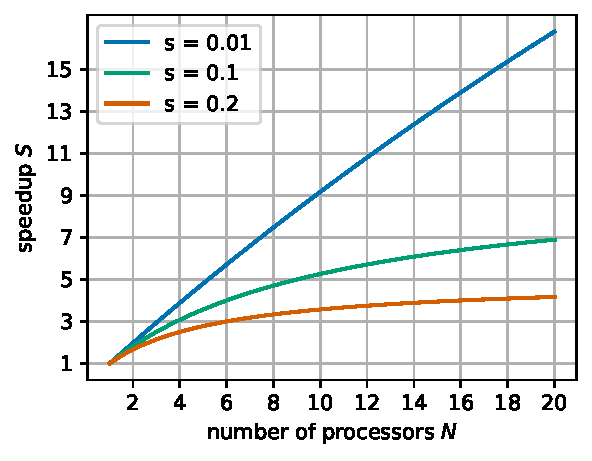
\includegraphics[width=0.9\textwidth]{figs/amdahl.pdf}
		%		%\caption{Speedup modeled by Amdahl's law for different portions of strictly serial workload}
		%		\label{fig:ideal_speedup}
		%	\end{figure}
		%\end{column}
	\end{columns}
\end{frame}

\begin{frame}
	\frametitle{Amdahl's Law}
	
	\begin{columns}
		\begin{column}{0.48\textwidth}
			In reality: several factors limiting parallelization: communication between processors, startup time, algorithmic limitations

			\vspace{10pt}

			Simple model given by \emph{Amdahl's law}
			\begin{equation}
				S = \frac{T_1}{T_N} = \frac{1}{s + \frac{1 - s}{N}}
			\end{equation}
			with \(s\) the part of the calculation which cannot be perfectly parallelized
		\end{column}

		\begin{column}{0.48\textwidth}
			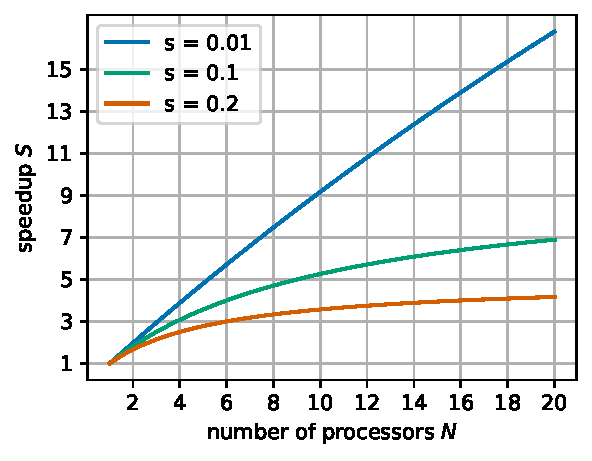
\includegraphics[width=0.9\textwidth]{figs/amdahl.pdf}
			\begin{itemize}
				\item upper bound for speedup given by \(\nicefrac{1}{s}\)
				\item smaller \(s\): closer to \(S = N\) for more processors
			\end{itemize}
			
		\end{column}
	\end{columns}
\end{frame}

\begin{frame}
	\frametitle{Solving the Kohn-Sham equations}

	\begin{columns}
	\begin{column}{0.5\textwidth}
	\centering
	\begin{tikzpicture}[
		scale=0.65,transform shape, squarednode/.style={rectangle, draw=purple!60, fill=purple!5, thick, minimum size=5mm, text centered, text width=8cm,},
		node distance=0.5cm]
		\tikzset{every node/.style={inner sep=8pt}}
		%Nodes
		\node[squarednode]      (init)          {Initial \(n(\vb*{r})\)};
		\node[squarednode]      (step_1)    [below= of init]  {Calculate \(v_{\mathrm{H}} [n(\vb*{r})]\) and \(v_{\mathrm{XC}} [n(\vb*{r})]\)};
		\node[squarednode]      (step_2)    [below= of step_1]      {Fourier transform potentials};
		\node[squarednode]      (step_3)    [below= of step_2]      {Solve Kohn-Sham equations in reciprocal space};
		\node[squarednode]      (step_4)    [below= of step_3]      {Fourier transform wave functions};
		\node[squarednode]      (step_5)    [below= of step_4]      {Calculate \(n(\vb*{r})\) and \(E [n(\vb*{r})]\)};
		\node[squarednode]      (done)      [below= of step_5]      {Done if change in \(E\) is small enough};
		
		%Lines
		\draw[->] (init.south) -- (step_1.north);
		\draw[->] (step_1.south) -- (step_2.north);
		\draw[->] (step_2.south) -- (step_3.north);
		\draw[->] (step_3.south) -- (step_4.north);
		\draw[->] (step_4.south) -- (step_5.north);
		\draw[->] (step_5.east) to [out=30,in=-30] (step_1.east);
		\draw[->] (step_5.south) -- (done.north);
	\end{tikzpicture}
	\end{column}

	\begin{column}{0.5\textwidth}
		Basis set for periodic systems: plane waves
		\begin{equation}
			\psi_{n \vb*{k}} (\vb*{r}) = \frac{1}{\sqrt{V}} \sum_{\vb*{G}} e^{i (\vb*{k} + \vb*{G}) \vb*{r}}
		\end{equation}	

		%\vspace{10pt}

		Multiple ways to parallelize:

		\begin{itemize}
			\item distributing grids in real/reciprocal space (\emph{R/G parallelization})
			\item solve Kohn-Sham equations for different \(k\)-points separately (\emph{\(k\)-point parallelization})
			\item (additionally in DFPT) separate calculations for different phonon wave vectors \(q\) (\emph{image parallelization})
		\end{itemize}
		
	\end{column}

	\end{columns}
\end{frame}

%\begin{frame}
%	\frametitle{DFPT calculations}
%
%	Phonon calculations are also possible within the framework of DFT

%	\vspace{10pt}

%	Task is again to solve a set of equations self-consistently, similar to the Kohn-Sham equations

%	Parallelization possibilities:
%		\begin{itemize}
%			\item Distributing grids in real/reciprocal space (enabled by default)
%			\item \(k\)-points parallelization
%			\item Split up calculations for different phonon wave vectors: \(q\)-point parallelization
%		\end{itemize}
%
%\end{frame}


\begin{frame}
	\frametitle{Parallelization parameters}

	\QE has the argument \texttt{nk}: determines number of processors pools the available processors are split into (for \(k\)-point parallelization)

	\(\implies\) different partition of the processors, depending on the total number of processors

	\vspace{8pt}
	\begin{columns}
		\begin{column}{0.5\textwidth}
			\centering
			no \(k\) point parallelization

			\centering
			
\includegraphics[width=0.3\textwidth]{figs/np16_no_kpoint.pdf}
			
			\centering
			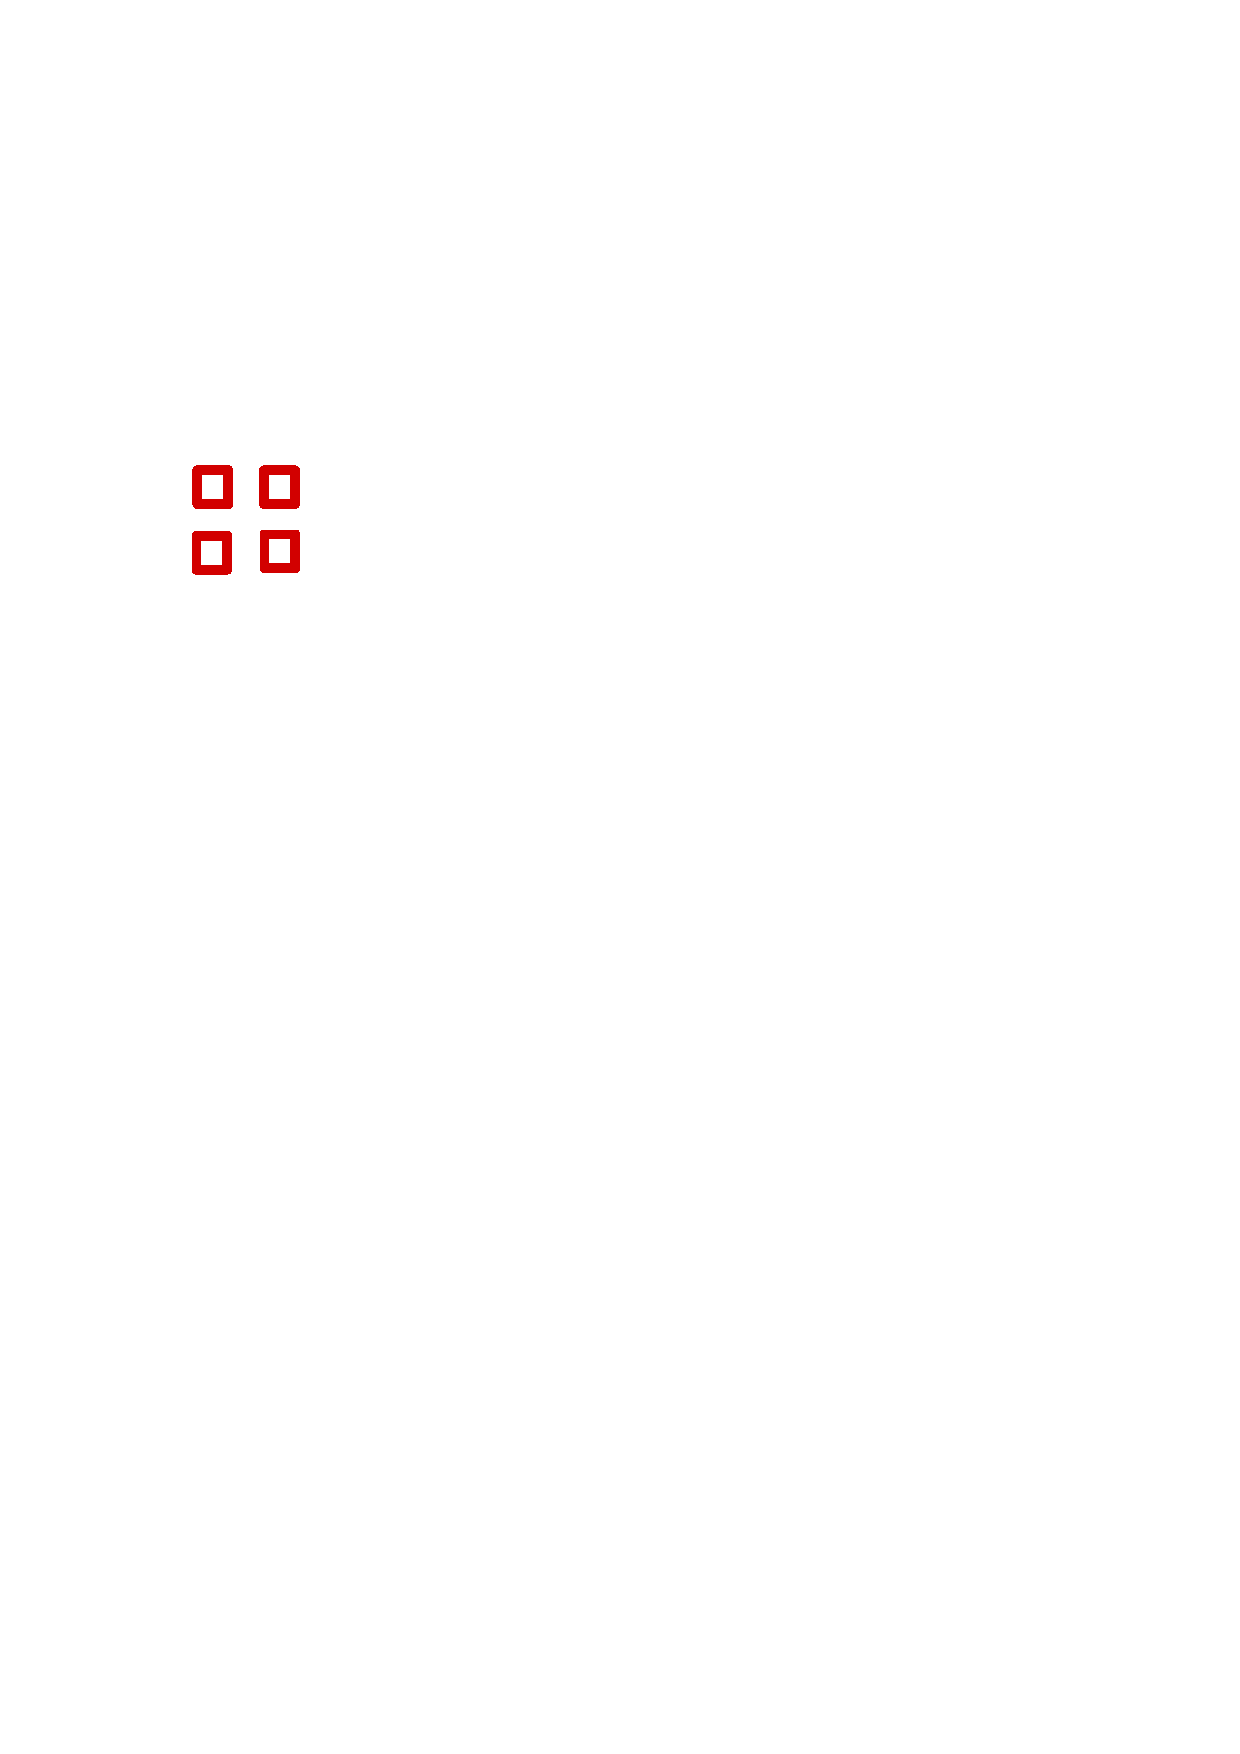
\includegraphics[width=0.15\textwidth]{figs/np4_no_kpoint.pdf}			
		\end{column}

		\begin{column}{0.5\textwidth}
			\centering
			\texttt{nk 4}

			\centering
			
\includegraphics[width=0.3\textwidth]{figs/np16_nk_4.pdf}			

			\centering
			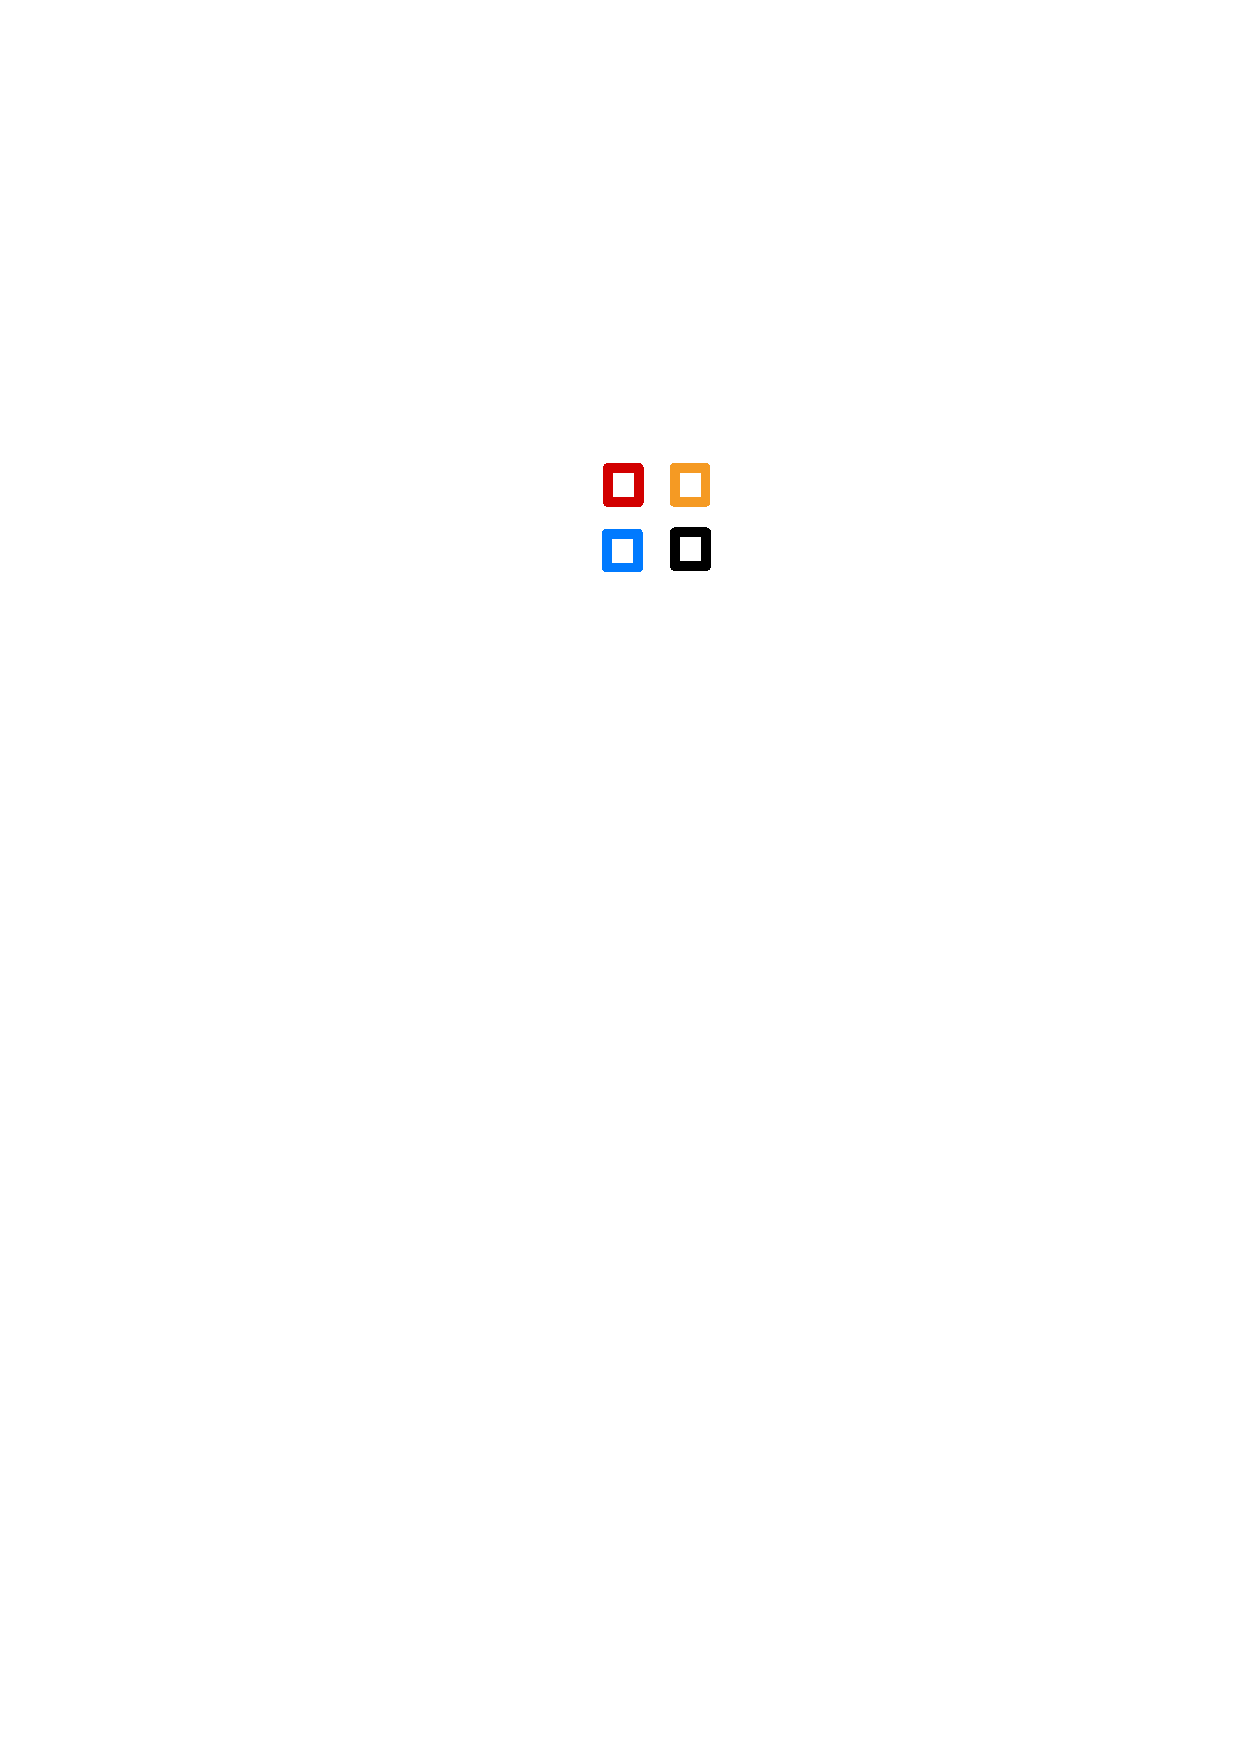
\includegraphics[width=0.15\textwidth]{figs/np4_nk_4.pdf}			
		\end{column}
	\end{columns}
	
	\vspace{8pt}

	Use size of the resulting pools for comparison, not the parameter \texttt{nk}

\end{frame}


\begin{frame}
	\frametitle{Examined system}

	\begin{columns}
		\begin{column}{0.5\textwidth}
			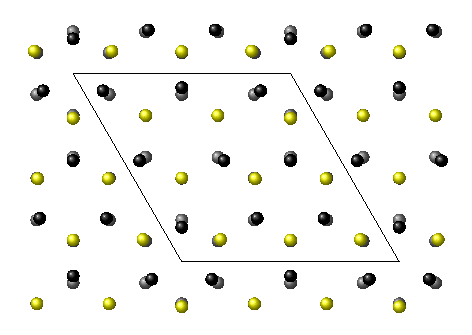
\includegraphics[width=\textwidth]{figs/symmetric.pdf}

			\centering
			light gray: symmetric structure

			dark gray/yellow: cdw structure
		\end{column}

		\begin{column}{0.5\textwidth}
			Monolayer Tantalum Disulfide (\TaS) in a \(3\times 3\) charge density wave
		\end{column}
	\end{columns}	

\end{frame}


% pwscf

\begin{frame}
	\begin{center}
		{\huge Benchmarking electronic structure calculations}
	\end{center}
\end{frame}

\begin{frame}
	\frametitle{No \(k\)-point parallelization}
	
	\begin{columns}
		\begin{column}{0.5\textwidth}
			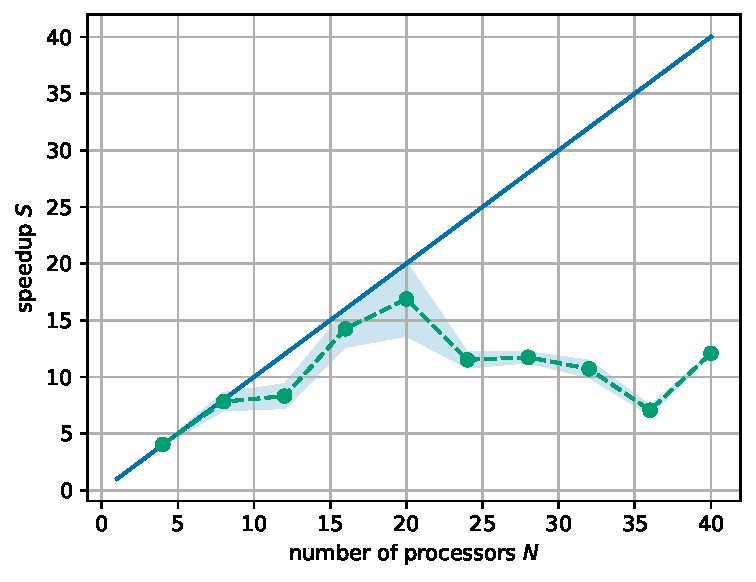
\includegraphics[width=0.9\textwidth]{figs/TaS2_ompi_bench_nprocs_speedup.pdf}
			\begin{itemize}
				\item OpenMPI/gcc compilers
				\item decline in speedup after 20 processors
			\end{itemize}
		\end{column}

		\begin{column}{0.5\textwidth}
				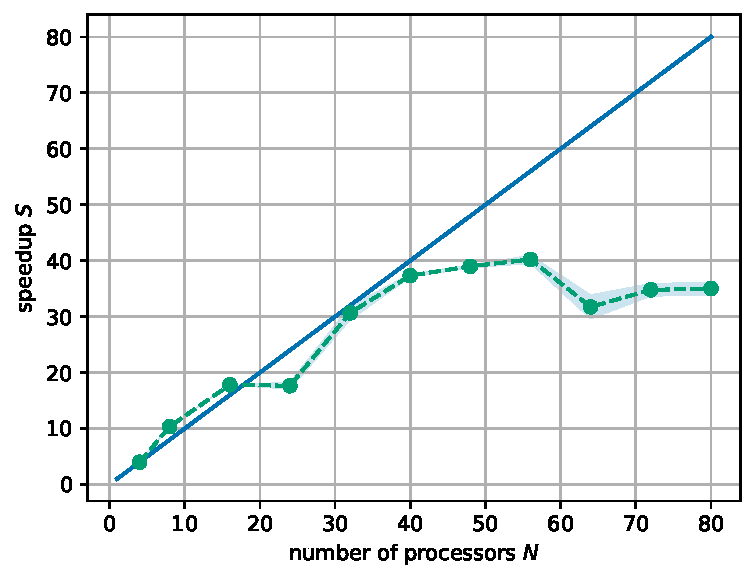
\includegraphics[width=0.9\textwidth]{figs/TaS2_intel_bench_nprocs_speedup.pdf}
			\begin{itemize}
				\item Intel compilers
				\item ideal speedup for up to 40 processors
			\end{itemize}
		\end{column}
	\end{columns}
\end{frame}


\begin{frame}
	\frametitle{\(k\)-point parallelization}
	
	\begin{columns}
		\begin{column}{0.5\textwidth}
			\begin{figure}
				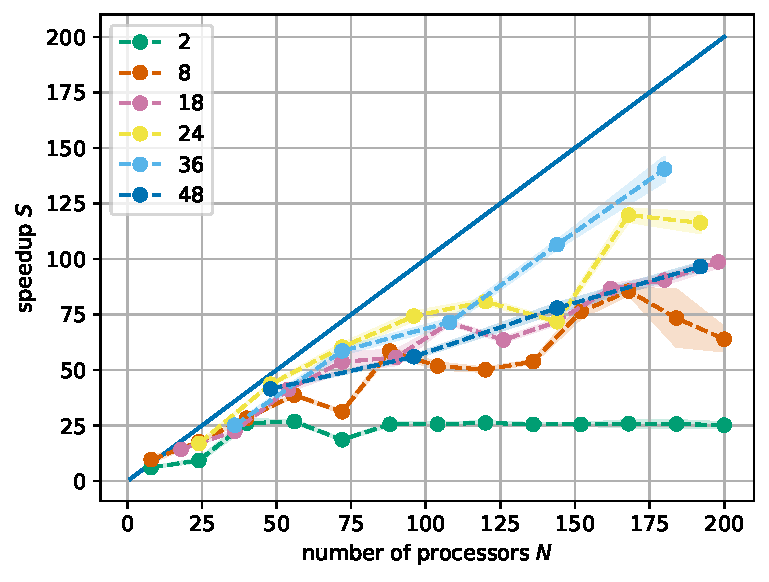
\includegraphics[width=\textwidth]{figs/TaS2_intel_bench_nk_speedup.pdf}
			\end{figure}
		\end{column}

		\begin{column}{0.5\textwidth}
			\begin{itemize}
				\item pool size 36 scales best
				\item consistent with the results of the benchmark without \(k\)-point parallelization
			\end{itemize}
		\end{column}
	\end{columns}

\end{frame}

\begin{frame}
	\frametitle{\(k\)-point parallelization}
	
	\begin{columns}
		\begin{column}{0.5\textwidth}
			\begin{figure}
				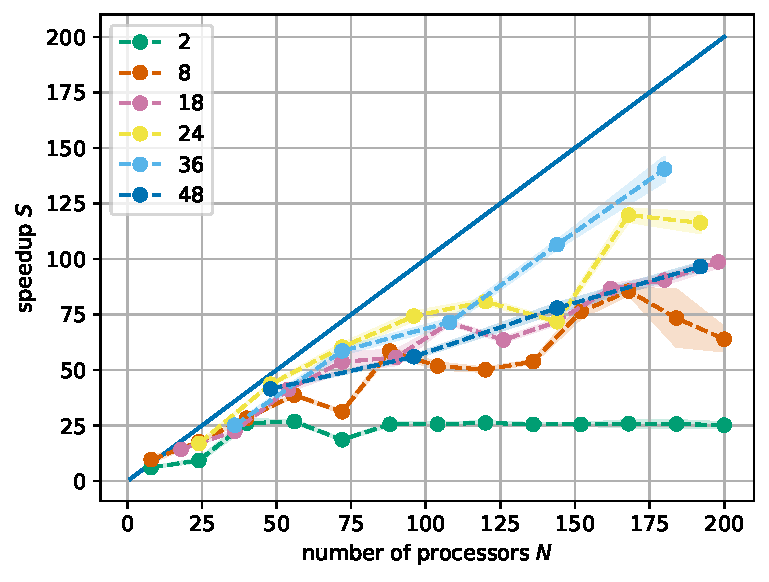
\includegraphics[width=\textwidth]{figs/TaS2_intel_bench_nk_speedup.pdf}
				\caption*{PHYSnet}
			\end{figure}
		\end{column}

		\begin{column}{0.5\textwidth}
			\begin{figure}
				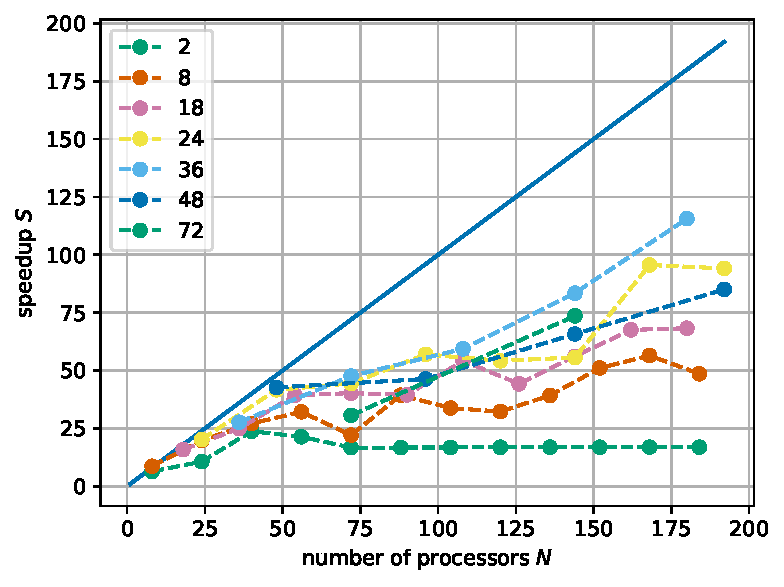
\includegraphics[width=\textwidth]{figs/TaS2_hlrn_bench_nk_speedup.pdf}
				\caption*{HLRN}
			\end{figure}
		\end{column}
	\end{columns}

\end{frame}


%\begin{frame}
%	\frametitle{\(k\)-point parallelization}
	
%	\begin{columns}
%		\begin{column}{0.5\textwidth}
%			\begin{figure}
%				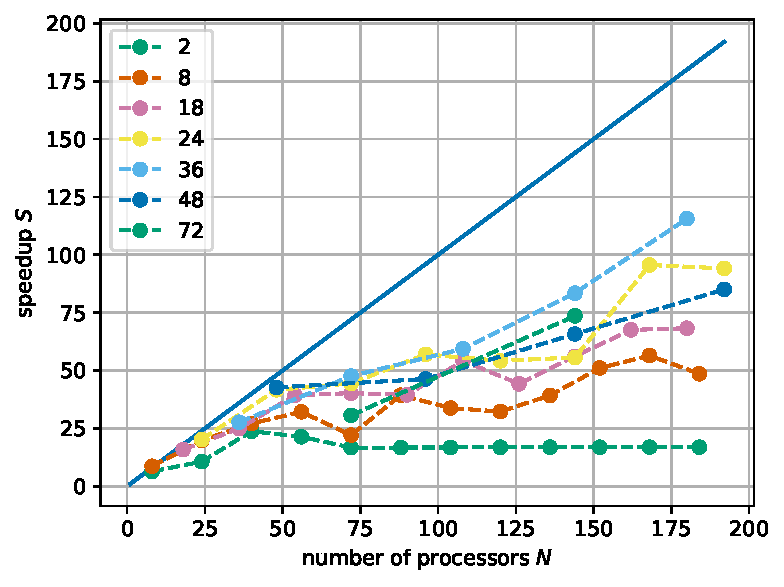
\includegraphics[width=\textwidth]{figs/TaS2_hlrn_bench_nk_speedup.pdf}
				%\caption*{HLRN}
			%\end{figure}
		%\end{column}
		%\begin{column}{0.5\textwidth}
			%\begin{itemize}
				%\item hardware topology is completely different: nodes have 96 cores each
				%\item pool size 36  still scales best
				%\item other pool sizes show a similar scaling as well
			%\end{itemize}	
		%\end{column}
	%\end{columns}

%\end{frame}

% Phonons

\begin{frame}
	\begin{center}
		{\huge Benchmarking phonon calculations}
	\end{center}
\end{frame}

\begin{frame}
	\frametitle{\(k\)-point parallelization}

	Two pool sizes tested, both on 180 processors:
	\begin{itemize}
		\item pool size 18: \SI{3044}{\minute}
    	\item pool size 36: \SI{2020}{\minute}
	\end{itemize}

	\vspace{10pt}

	Difference already after first phonon mode:
	\begin{itemize}
		\item pool size 18: \SI{2832.1}{\second}
		\item pool size 36: \SI{2183.3}{\second}
	\end{itemize}
\end{frame}

%\begin{frame}
%	\frametitle{Image parallelization}
%
%	\begin{columns}
%		\begin{column}{0.5\textwidth}
%			\begin{figure}
%				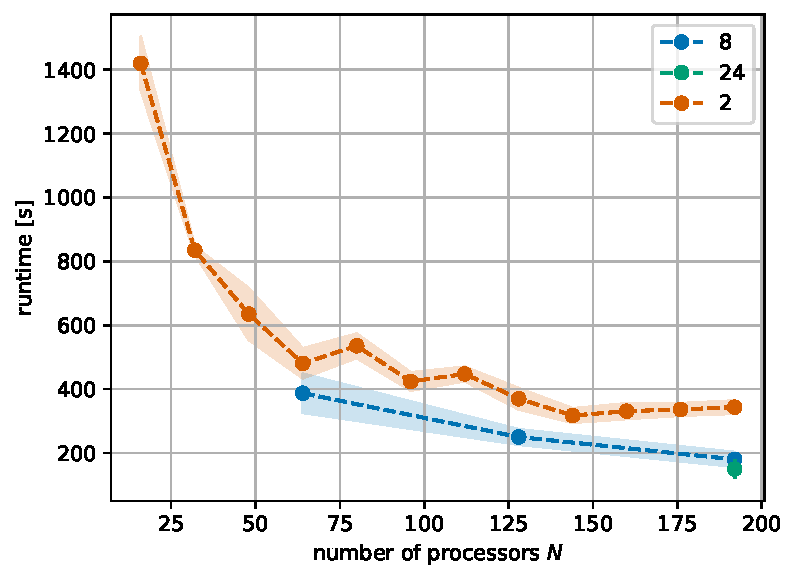
\includegraphics[width=\textwidth]{figs/si_ph_poolsize_8_images_distribution.pdf}
%			\end{figure}
%		\end{column}
%
%		\begin{column}{0.5\textwidth}
%			\begin{itemize}
%				\item 
%			\end{itemize}
%		\end{column}
%	\end{columns}
%
%\end{frame}

\begin{frame}
	\frametitle{Image parallelization}

	\begin{columns}
		\begin{column}{0.5\textwidth}
			\begin{figure}
				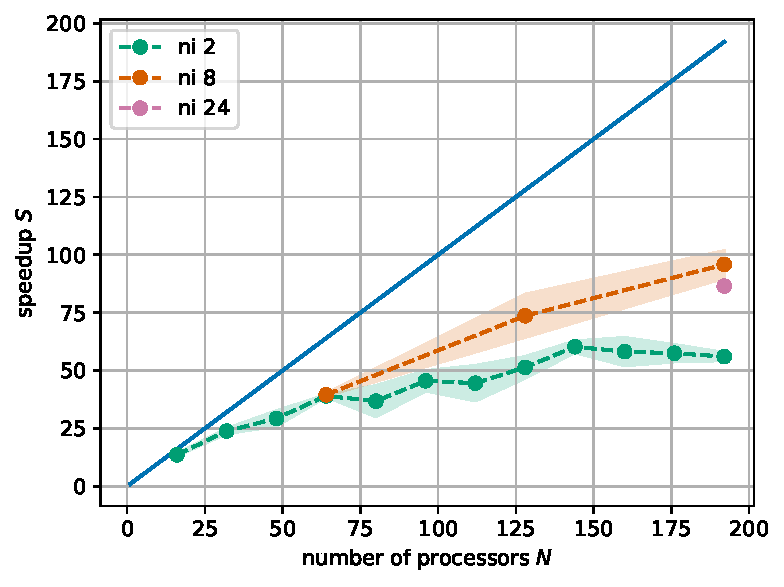
\includegraphics[width=\textwidth]{figs/si_ph_poolsize_8_bench_ni_speedup.pdf}
			\end{figure}
		\end{column}

		\begin{column}{0.5\textwidth}
			\begin{itemize}
				\item benchmark run on bulk silicon
				\item different combinations of \texttt{ni} (different colors in the plot) and \texttt{nk} with resulting pool size of 8
				\item linear scaling continues when using more images
			\end{itemize}
		\end{column}
	\end{columns}

\end{frame}


% Conclusion

\begin{frame}
	\frametitle{Conclusion}


	\begin{columns}
		\begin{column}{0.5\textwidth}
			\begin{itemize}
				\item Right choice of parallelization parameters has a significant impact on the runtime of calculations with \QE
				\item Good choice of parameters translates between the two modules examined as well as between different compute clusters
			\end{itemize}
		\end{column}
		\begin{column}{0.5\textwidth}
			\begin{figure}
				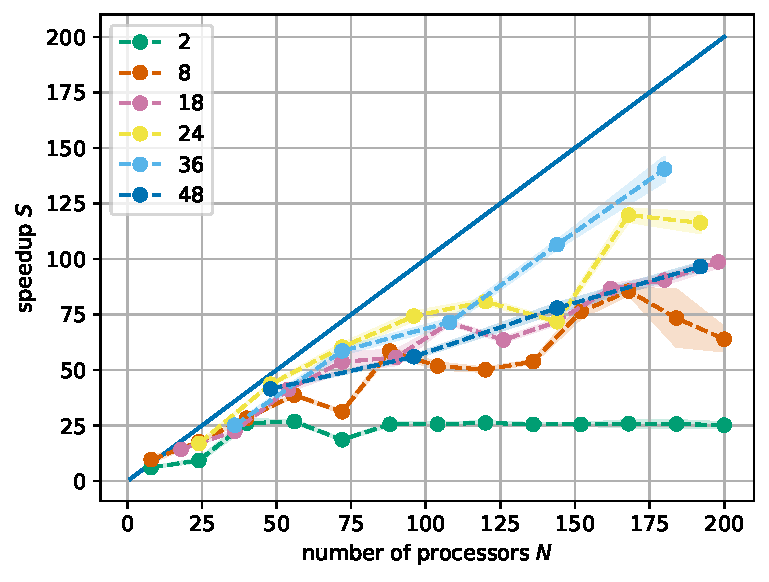
\includegraphics[width=\textwidth]{figs/TaS2_intel_bench_nk_speedup.pdf}
				\caption*{PHYSnet}
			\end{figure}
		\end{column}
	\end{columns}

\end{frame}

% Folien für Rückfragen

%\appendix
\begin{frame}
	\centering
	{\huge Additional slides}
\end{frame}

%\begin{frame}
%	\frametitle{Factors limiting parallel execution}
%\end{frame}

\begin{frame}
	\frametitle{\(k\) point parallelization: Memory}

	Electronic structure calculations on \TaS, 180 processors

	\vspace{10pt}

	pool size 18:
	\begin{itemize}
		\item Estimated max dynamical RAM per process > 178.04 MB
		\item Estimated total dynamical RAM > 28.67 GB
	\end{itemize}

	pool size 36:
	\begin{itemize}
		\item Estimated max dynamical RAM per process > 103.76 MB
		\item Estimated total dynamical RAM > 17.07 GB
	\end{itemize}
\end{frame}

\begin{frame}
	\frametitle{Electronic structure calculations}

	\centering
	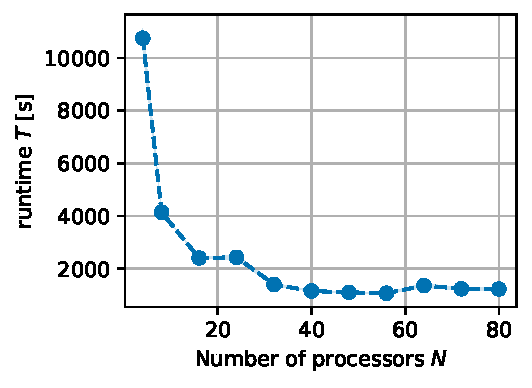
\includegraphics[width=0.6\textwidth]{figs/TaS2_intel_bench_nprocs_absolute.pdf}

\end{frame}

\begin{frame}
	\frametitle{Linear Algebra parallelization}
\end{frame}

%\begin{frame}
%	\frametitle{Compilers?}

%	Intel

%	OpenMPI

%\end{frame}

\begin{frame}
	\frametitle{Amdahl's Law}
	
	\begin{columns}
		\begin{column}{0.48\textwidth}
			%\vspace{10pt}
			Simple model given by \emph{Amdahl's law}:
			\begin{itemize}
				\item split serial time into serial part \(s\) and perfectly parallelizable part \(p\): 
				\begin{equation}
					T_1 = s + p = 1
				\end{equation}	
				\item execution time on \(N\) processors: 
				\begin{equation}
					T_N = s + \frac{p}{N}
				\end{equation}
				\item speedup: 
				\begin{equation}
					S = \frac{T_1}{T_N} = \frac{1}{s + \frac{p}{N}} = \frac{1}{s + \frac{1 - s}{N}}
				\end{equation}
			\end{itemize}
		\end{column}

		\begin{column}{0.48\textwidth}
			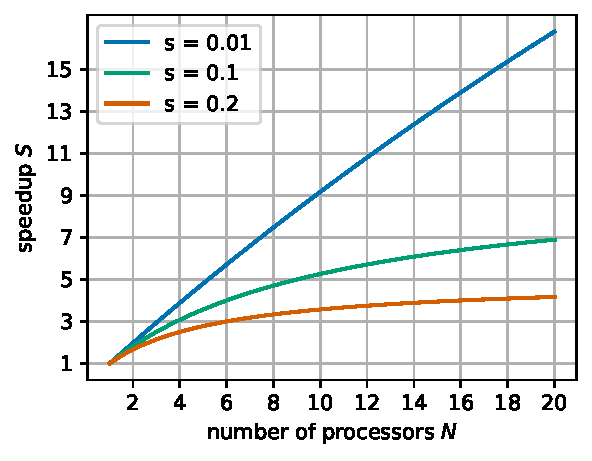
\includegraphics[width=0.9\textwidth]{figs/amdahl.pdf}
			\begin{itemize}
				\item upper bound for speedup given by \(\nicefrac{1}{s}\)
				\item smaller \(s\): closer to \(S = N\) for more processors
			\end{itemize}
			
		\end{column}
	\end{columns}
\end{frame}

\end{document}
